\subsection{SymPy Gamma}\label{sympy-gamma}

SymPy Gamma is a simple web application that runs on Google App Engine. 
It executes and displays the results of SymPy expressions as well as
additional related computations, in a fashion similar to that of
Wolfram\textbar{}Alpha. For instance, entering an integer will display
its prime factors, digits in the base-10 expansion, and a factorization
diagram. Entering a function will display its docstring; in general,
entering an arbitrary expression will display its derivative, integral,
series expansion, plot, and roots.

SymPy Gamma also has several additional features than just computing the
results using SymPy.

\begin{itemize}
\item
  It displays integration steps, differentiation steps in detail, which
  can be viewed in Figure \ref{fig:integralsteps}:\par
\begin{minipage}{\textwidth}
    \centering
    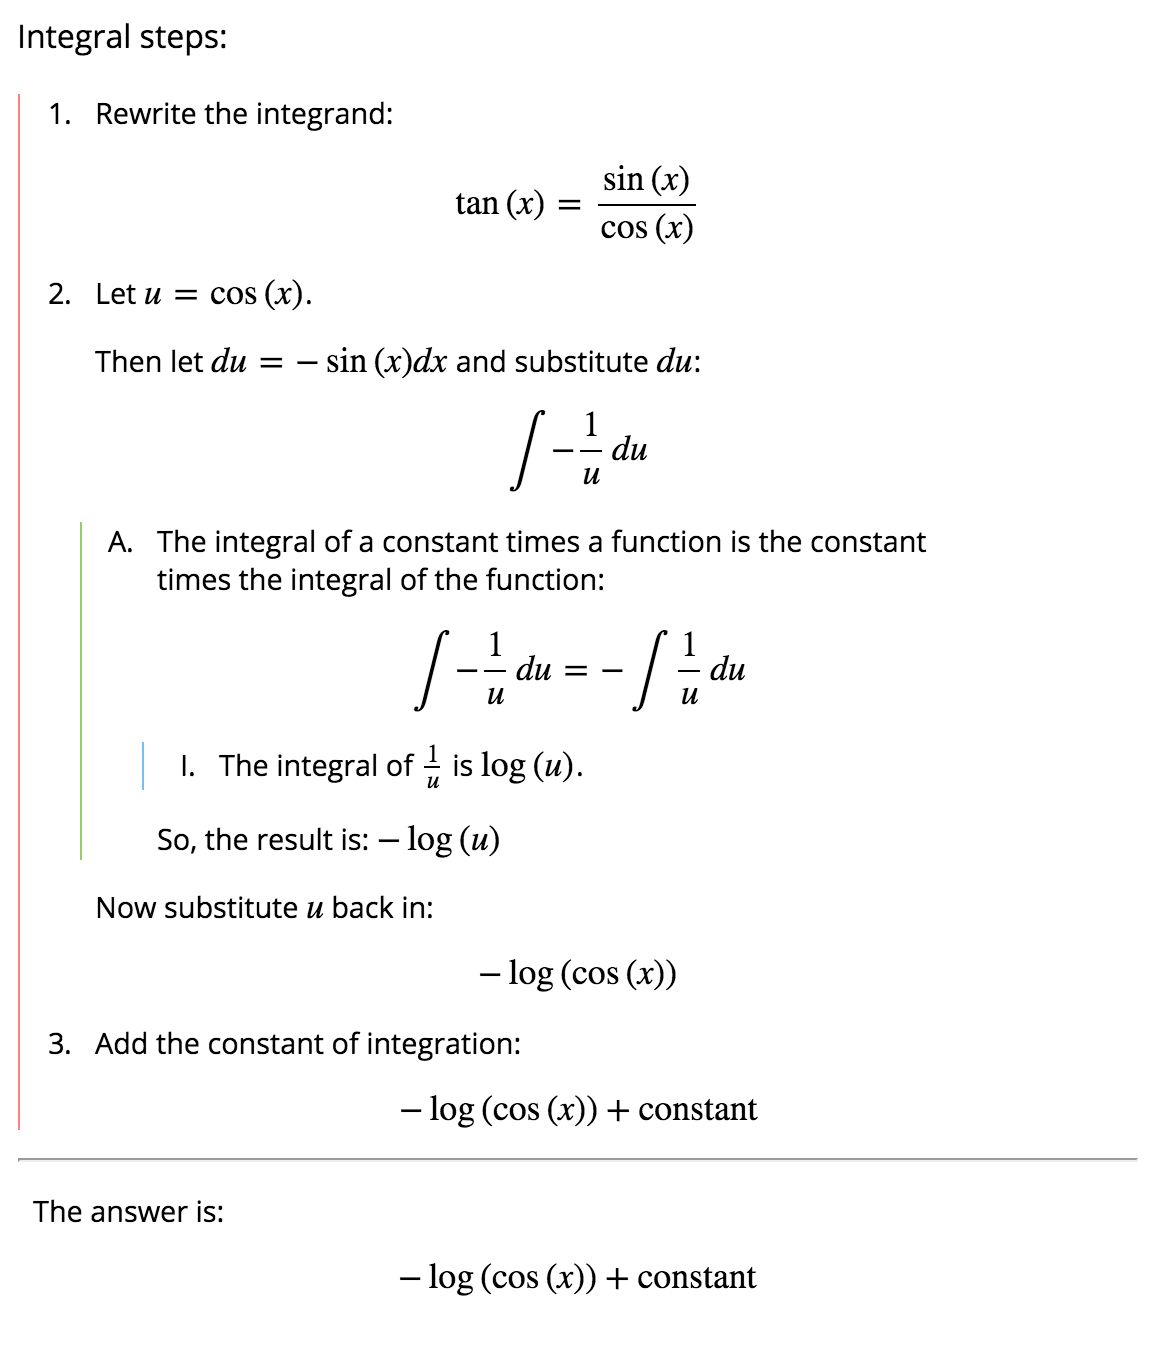
\includegraphics[width=0.7\textwidth]{integral_steps.png}
    \captionof{figure}{Integral steps of $\tan (x)$}
    \label{fig:integralsteps}
\end{minipage}
\item
  It also displays the factor tree diagrams for different numbers.
\item
  SymPy Gamma also saves user search queries, and offers many such 
  similar features for free, which Wolfram\textbar{}Alpha only offers 
  to its paid users.
\end{itemize}
Every input query from the user on SymPy Gamma is first, parsed by its
own parser, which handles several different forms of function names,
which SymPy as a library doesn't support. For instance, SymPy Gamma
supports queries like \texttt{sin\ x}, whereas SymPy doesn't support
this, and supports only \texttt{sin(x)}.

This parser converts the input query to the equivalent SymPy readable 
code, which is then eventually processed by SymPy and the result is 
finally formatted in LaTeX and displayed on the SymPy Gamma web-application.

\subsection{SymPy Live}\label{sympy-live}

SymPy Live is an online Python shell, which runs on Google
App Engine, that executes SymPy code. It is integrated in the SymPy
documentation examples, located at this \href{http://docs.sympy.org/latest/index.html}{link}.

This is accomplished by providing a HTML/JavaScript GUI for entering
source code and visualization of output, and a server part which
evaluates the requested source code. It's an interactive AJAX shell,
that runs SymPy code using Python on the server.
\newline
Certain Features of SymPy Live-:

\begin{itemize}
\item
  It supports the exact same syntax as SymPy, hence it can be used
  easily, to test for outputs of various SymPy expressions.
\item
  It can be run as a standalone app or in an existing app as an
  admin-only handler, and can also be used for system administration
  tasks, as an interactive way to try out APIs, or as a debugging aid
  during development.
\item
  It can also be used to plot figures (\href{http://live.sympy.org/?evaluate=from\%20sympy\%20import\%20symbols\%0Afrom\%20sympy.plotting\%20import\%20textplot\%0Ax\%20\%3D\%20symbols(\%27x\%27)\%0Atextplot(x**2\%2C0\%2C5)\%0A\%23--\%0A}{link}), 
  and execute all kinds of expressions that SymPy can evaluate.
\item
SymPy Live also formats the output in LaTeX for pretty-printing the
output.
\end{itemize}